%  Beamer slide example.

\documentclass[9pt]{beamer}
%\setbeameroption{show only notes}
%\setbeameroption{show notes}

\usepackage[utf8]{inputenc}
\usetheme{inria}
\usepackage{helvet}
\usepackage{graphicx}

\usepackage{tikz}
\usetikzlibrary{arrows,shapes,positioning,calc,shadows,trees}
\tikzset{
  mstep1/.style = {basic, rounded corners=2pt, thin, align=center, fill=orange!70,text width=1.5cm},
  mstep2/.style = {basic, rounded corners=2pt, thin, align=center, fill=green!30,text width=1.5cm},
  mstep2b/.style = {basic, rounded corners=2pt, thin, align=center, fill=white,text width=2cm},
  mstep3/.style = {basic, rounded corners=2pt, thin, align=center, fill=green!30,text width=3cm},
  mstep3b/.style = {basic, rounded corners=2pt, thin, align=center,fill=white,text width=7cm},
  mstep4/.style = {basic, thin, align=left, fill=gray!60, text width=6.5em},
  basic/.style  = {draw, text width=2cm, drop shadow, font=\sffamily, rectangle},
  root/.style   = {basic, rounded corners=2pt, thin, align=center,
  fill=green!30},
  level 2/.style = {basic, rounded corners=6pt, thin,align=center, fill=green!60,
  text width=8em},
  level 3/.style = {basic, thin, align=left, fill=orange!60, text width=6.5em},
  mlevel4/.style = {basic, thin, align=left, fill=gray!60, text width=6.5em}
}
\tikzstyle{every picture}+=[remember picture]
\tikzstyle{na} = [baseline=-.5ex]


\def\aboxl[#1,#2,#3,#4,#5]#6{%
  \node[draw, cylinder, alias=cyl, shape border rotate=90, aspect=#3, %
    minimum height=#1, minimum width=#2, outer sep=-0.5\pgflinewidth, %
    color=orange!40!black, left color=orange!70, right color=orange!80, middle
  color=white] (#4) at #5 {};%
  \node at #5 {#6};%
  \fill [orange!30] let \p1 = ($(cyl.before top)!0.5!(cyl.after top)$), \p2 =
  (cyl.top), \p3 = (cyl.before top), \n1={veclen(\x3-\x1,\y3-\y1)},
\n2={veclen(\x2-\x1,\y2-\y1)} in (\p1) ellipse (\n1 and \n2); }

\author{Maurice Brémond \and Gaëtan Harter}

\title[Intégration continue]{L'Intégration Continue}
% \subtitle{Dans un contexte de développement Inria}
\subtitle{Présentation IJD}

% Automatically insert a "new section" page at each section.
\AtBeginSection[]{
  \begin{frame}[plain]
    \partpage
  \end{frame}
}
% \inriaswitchcolors COLOR
%
% Where COLOR is one of red, blue, orange, darkblue, violet,
% pastelgreen, grey, or green.
\newcommand{\inriaswitchcolors}[1]{%
  \pgfaliasimage{figfootline}{figfootline-#1}% !!!
  \pgfaliasimage{figbackground}{figbackground-#1}% !!!
  \pgfaliasimage{figbackground}{figbackground-#1}% !!!
}

% frame with toc for current subsection
\newcommand{\tocsubsection}[1]{
  \begin{frame}
    \tableofcontents[
      currentsubsection,
      sectionstyle=show/shaded,
      subsectionstyle=show/shaded,
      subsubsectionstyle=show/show/shaded
    ]
    #1
  \end{frame}
}
% starting the document
% *********************
\begin{document}

% titlepage
% ---------
\begin{frame}[plain]
  \titlepage
\end{frame}
% table of contents
% -----------------
\begin{frame}{\textcolor{inriaGrey}{Table des matières}}
  \tableofcontents
\end{frame}



% Introduction
% ************

\inriaswitchcolors{red}
\section{Quid de l'intégration continue}

\subsection{Définition}

\begin{frame}{En quelques mots}
\begin{block}{Le processus d'intégration d'un logiciel : une chaine de production}
\begin{tikzpicture}
  \node[] (developer1) {
\includegraphics[width=.04\textwidth] {images/Laptop-icon.png}};
  \node[below=.001cm of developer1] (developer2) {
\includegraphics[width=.04\textwidth] {images/Laptop-icon.png}};
  \node[below=.001cm of developer2] (developer3) {
\includegraphics[width=.04\textwidth] {images/Laptop-icon.png}};
  \node[right=1.3cm of developer2] (code_repo_db) {};
  \node[above=.4cm of code_repo_db] (code_repo_db_north) {};
  \node[left=.2cm of code_repo_db] (code_repo_db_west) {};
  \node[below=.1cm of code_repo_db] (code_repo_db_south) {};
  \node[below=.9cm of code_repo_db,mstep1] (code_repo) {gestion de versions};
  \aboxl[25,20,1.6,a1,(code_repo_db)] {};
  \node[right=.6cm of code_repo,mstep2] (build) {production (``build'')};
  \node[above=.4cm of build] (nux) {
\includegraphics[width=.04\textwidth] {images/Linux-icon.png}};
  \node[above=.001cm of nux] (windows) {
\includegraphics[width=.04\textwidth] {images/Windows-icon.png}};
  \node[above=.001cm of windows] (freebsd) {
\includegraphics[width=.04\textwidth] {images/Apps-freebsd-icon.png}};
  \node[right=.6cm of build,mstep2] (tests) {tests};
  \node[above=.4cm of tests] (test_ok1) {
\includegraphics[width=.02\textwidth] {images/accept-icon.png}};
  \node[above=.001cm of test_ok1] (test_ok2) {
\includegraphics[width=.02\textwidth] {images/accept-icon.png}};
  \node[above=.001cm of test_ok2] (test_bad1) {
\includegraphics[width=.02\textwidth] {images/delete-icon.png}};
  \node[above=.001cm of test_bad1] (test_ok4) {
\includegraphics[width=.02\textwidth] {images/accept-icon.png}};
  \node[right=.001cm of test_ok1] (test_bad1) {
\includegraphics[width=.02\textwidth] {images/delete-icon.png}};
  \node[right=.001cm of test_ok2] (test_ok3) {
\includegraphics[width=.02\textwidth] {images/accept-icon.png}};
  \node[right=.6cm of tests,mstep2] (install) {installation paquetage};
  \node[above=.4cm of install] (package) {
\includegraphics[width=.06\textwidth] {images/System-Package-icon.png}};
  \path[<->, thick, color=blue] (developer1) edge [bend left] (code_repo_db_north);
  \path[<->, thick, color=blue] (developer2) edge [] (code_repo_db_west);
  \path[<->, thick, color=blue] (developer3) edge [bend right] (code_repo_db_south);
  \path[->, thick, color=gray,dotted] (code_repo.east) edge [] (build.west);
  \path[->, thick, color=gray,dotted] (build) edge [] (tests);
  \path[->, thick, color=gray,dotted] (tests) edge [] (install);
\end{tikzpicture}
\end{block}
\begin{block}{En ``continu''}
\begin{itemize}
\item Une nouvelle contribution met en oeuvre toute la chaine de production
\item et/ou régulièrement : intégration nocturne, hebdomadaire
\end{itemize}
\end{block}
\end{frame}

\subsection{Pourquoi et ce que cela implique}

\begin{frame}{Intégration continue}

  \begin{block}{Pourquoi ?}
    Un cycle court pour traiter au plus tôt les problèmes
    \begin{itemize}
    \item les régressions dans les tests
    \item les régressions dans la portabilité
    \item les codes difficiles à fusionner
    \item \dots
  \end{itemize}

  \textbf{L'intégration continue est liée à une méthode de travail}

\end{block}

\begin{block}{Ce que cela implique :}
\begin{itemize}
\item les différentes étapes de la chaine doivent être \textbf{automatisées} : production, tests, paquetage
\item un moteur doit permettre de déclencher chaque étape
\item une synthèse des résultats doit être disponible
\end{itemize}
\end{block}
\end{frame}

\subsection{Problématiques autour des automatisations nécessaires}
\begin{frame}{Automatisation de l'étape de production}
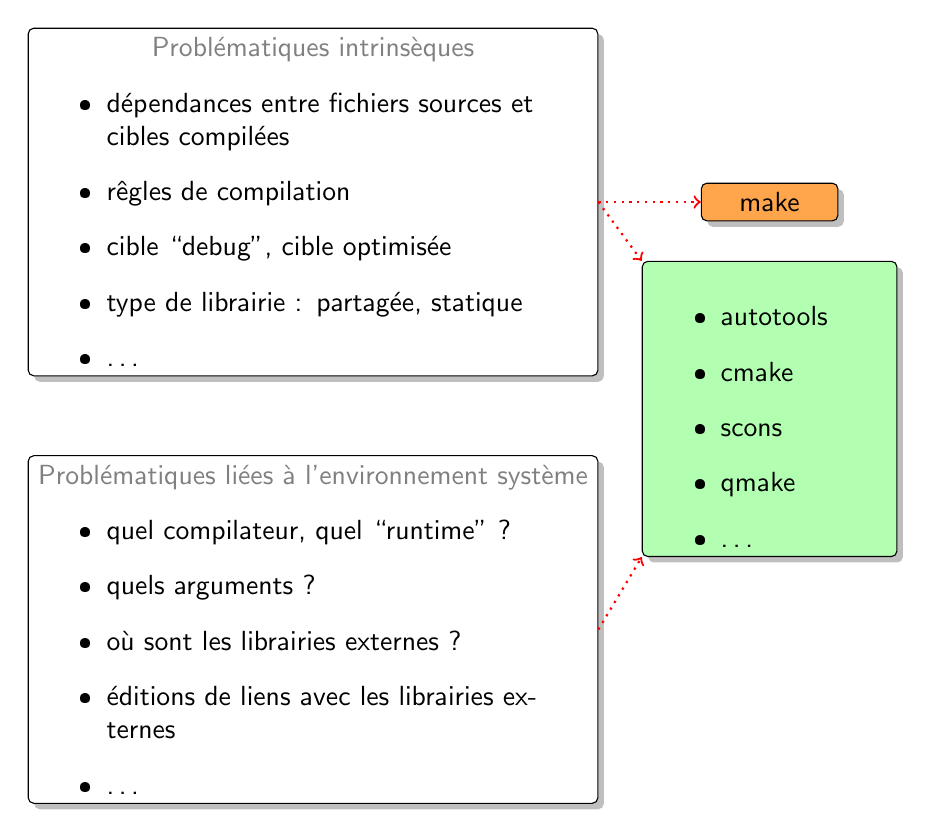
\begin{tikzpicture}
\node[mstep3b] (intrinsics) {
\textcolor{gray}{Problématiques intrinsèques}
  \begin{itemize}
  \item dépendances entre fichiers sources et cibles compilées
  \item rêgles de compilation
  \item cible ``debug'', cible optimisée
  \item type de librairie : partagée, statique
  \item \dots
  \end{itemize}};
\node[below=1cm of intrinsics,mstep3b] (extrinsics) {
\textcolor{gray}{ Problématiques liées à l'environnement système}
  \begin{itemize}
  \item quel compilateur, quel ``runtime'' ?
  \item quels arguments ?
  \item où sont les librairies externes ?
  \item éditions de liens avec les librairies externes
  \item \dots
  \end{itemize}};
\node [right=1.3cm of intrinsics,mstep1] (make) {make};
\node [below=.5cm of make,mstep3] (build_tools) {
  \begin{itemize}
  \item autotools
  \item cmake
  \item scons
  \item qmake
  \item \dots
  \end{itemize}};

\node[above=.1cm of build_tools] (build_tools_north) {};
\node[below=.1cm of build_tools] (build_tools_south) {};
\path[->, thick, color=red,dotted] (intrinsics.east) edge [] (make.west);
\path[->, thick, color=red,dotted] (intrinsics.east) edge [] (build_tools.north west);
\path[->, thick, color=red,dotted] (extrinsics.east) edge [] (build_tools.south west);
\end{tikzpicture}
\end{frame}

\begin{frame}{Les tests : problématiques et outils}

%
%    2.1 Maintain a code repository
%    2.2 Automate the build
%    2.3 Make the build self-testing
%    2.4 Everyone commits to the baseline every day
%    2.5 Every commit (to baseline) should be built
%    2.6 Keep the build fast
%    2.7 Test in a clone of the production environment
%    2.8 Make it easy to get the latest deliverables
%    2.9 Everyone can see the results of the latest build
%    2.10 Automate deployment
%

  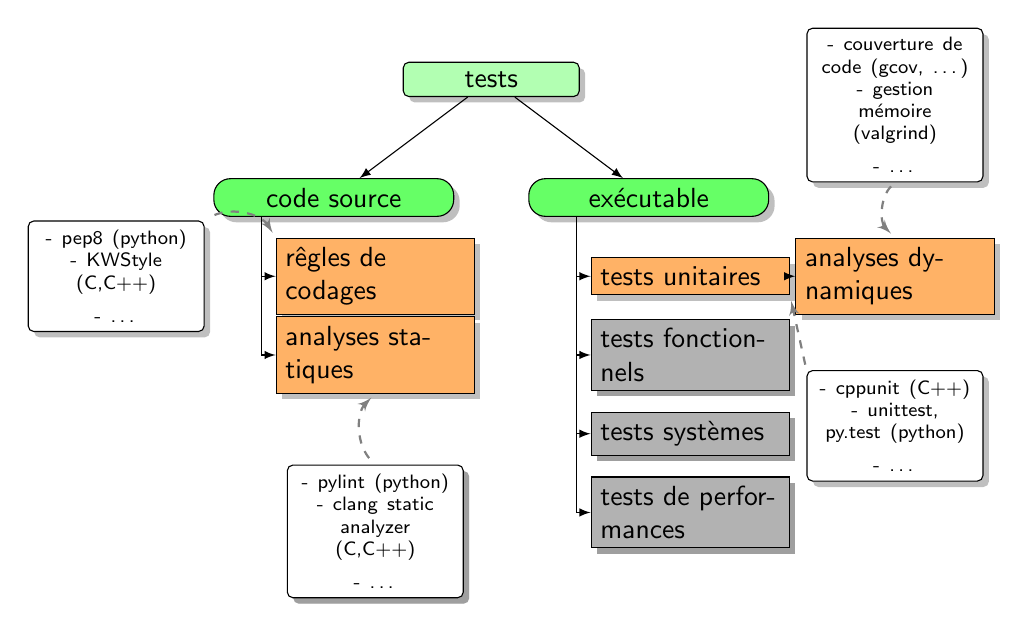
\begin{tikzpicture}[
      level 1/.style={sibling distance=40mm},
      edge from parent/.style={->,draw},
    >=latex]

% root of the the initial tree, level 1
    \node[root] {tests}
% The first level, as children of the initial tree
    child {node[level 2] (c1) {code source}}
    child {node[level 2] (c2) {exécutable}};


% The second level, relatively positioned nodes
    \begin{scope}[every node/.style={level 3}]
      \node [below of = c1, xshift=15pt] (c11) {rêgles de codages};
      \node [below of = c11] (c12) {analyses statiques};
      \node [below of = c2, xshift=15pt] (c21) {tests unitaires};
      \node [below of = c21,mstep4] (c22) {tests fonctionnels};
      \node [below of = c22,mstep4] (c23) {tests systèmes};
      \node [below of = c23,mstep4] (c24) {tests de performances};
      \node [right of = c21,xshift=1.6cm] (dynamic_analysis) {analyses dynamiques};
      \node [below=.9cm of c12,mstep2b] (static_an) {\scriptsize
        - pylint (python) \\
        - clang static analyzer (C,C++) \\
        - \dots
      };
    \end{scope}
      \node[left=.9cm of c11,mstep2b] (codage) {\scriptsize
        - pep8 (python)  \\
        - KWStyle (C,C++) \\
        - \dots
      };
      \node[above=.7cm of dynamic_analysis,mstep2b] (dynamic_analysis_tools) {\scriptsize
        - couverture de code (gcov, \dots) \\
        - gestion mémoire (valgrind) \\
        - \dots
      };
      \node[below=.7cm of dynamic_analysis,mstep2b] (unit_tests_tools) {\scriptsize
        - cppunit (C++) \\
        - unittest, py.test (python) \\
        - \dots
      };
      \draw[<-, >=latex', shorten >=2pt, shorten <=2pt, thick, color=gray, bend right=45,dashed]
      (c11.north west) to node[auto, swap] {} (codage.north east);
      \draw[<-, >=latex', shorten >=2pt, shorten <=2pt, thick, color=gray, bend right=45,dashed]
      (c12.south) to node[auto, swap] {} (static_an.north);
      \draw[->, >=latex', shorten >=2pt, shorten <=2pt, thick, color=gray, bend right=45,dashed]
      (dynamic_analysis_tools.south) to node[auto, swap] {} (dynamic_analysis.north);
      \draw[->, >=latex', shorten >=2pt, shorten <=2pt, thick, color=gray,dashed]
      (unit_tests_tools.north west) to node[auto, swap] {} (c21.south east);

% lines from each level 1 node to every one of its "children"
    \draw[->] (c21.east) |- (dynamic_analysis.west);

    \foreach \value in {1,2}
    \draw[->] (c1.195) |- (c1\value.west);

    \foreach \value in {1,...,4}
    \draw[->] (c2.195) |- (c2\value.west);


    % \node [draw,rectangle,fill=gray] at (8,0) {Intégration continue}
    % child {node [draw,rectangle,fill=gray] {compilations automatiques}}
    % child {node [draw,rectangle,fill=gray] {tests automatiques}}
    % child {node [draw,rectangle,fill=gray] {``commits'' journaliers}}
    % child {node [draw,rectangle,fill=gray] {tous les ``commits'' doivent être compilés et testés}}
    % child {node [draw,rectangle,fill=gray] {la compilation doit rester rapide}}
    % child {node [draw,rectangle,fill=gray] {le test ne doit pas se faire dans l'environnement de production}}
    % child {node [draw,rectangle,fill=gray] {les résultats des dernières compilations et tests doivent être visibles}}
    % child {node [draw,rectangle,fill=gray] {le déploiement doit être automatisé}};


   % \node[draw,rectangle,color=black] {Intégration continue}
   % node[] {dépôt du code source \textbf{versionné}}
   % child { node[] {compilations automatiques} }
   % child { node[] {tests automatiques} }
   % child { node[] {``commits'' journaliers} }
   % child { node[] {tous les ``commits'' doivent être compilés} }
   % child { node[] {la compilation doit rester rapide} }
   %    child { node[] {le test ne doit pas se faire dans l'environnement de production} }
   %    child { node[] {le dernier délivrable doit être disponible facilement} }
   %    child { node[] {les résultats des dernières compilations et tests doivent être visibles} }
   %    child { node[] {le déploiement doit être automatisé} }
   %  } ;
  \end{tikzpicture}

\end{frame}

\begin{frame}{Une orchestration}
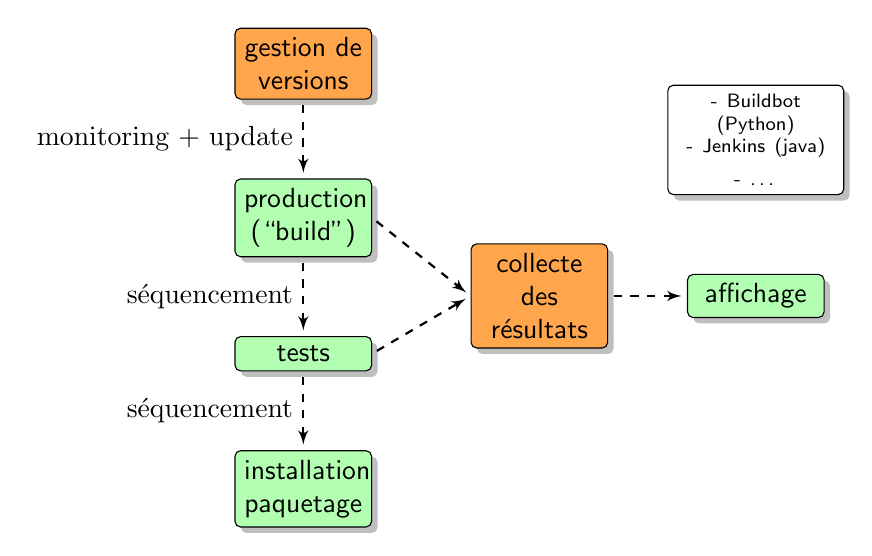
\begin{tikzpicture}
%  \node[mstep1] (integ) { Intégration continue };
  \node[mstep1] (code_repo) {gestion de versions};
  \node[below=1cm of code_repo,mstep2] (build) {production (``build'')};
  \node[below=1cm of build,mstep2] (tests) {tests};
  \node[below=1cm of tests,mstep2] (install) {installation paquetage};
  \node[right=2cm of build] (build_r1) {};
  \node[below=.2cm of build_r1,mstep1] (build_r) {collecte des résultats};
  \node[right=1cm of build_r,mstep2] (build_r_a) {affichage};
  \node[above=1cm of build_r_a,mstep2b] (tools) {\scriptsize - Buildbot (Python) \\
  - \alert{Jenkins} (java) \\
  - \dots};
  \draw[->, >=latex', shorten >=2pt, shorten <=2pt, thick, dashed]
  (code_repo.south) to node[auto, swap] {monitoring + update} (build.north);
  \draw[->, >=latex', shorten >=2pt, shorten <=2pt, thick, dashed]
  (build.south) to node[auto, swap] {séquencement} (tests.north);
  \draw[->, >=latex', shorten >=2pt, shorten <=2pt, thick, dashed]
  (tests.south) to node[auto, swap] {séquencement} (install.north);
  \draw[->, >=latex', shorten >=2pt, shorten <=2pt, thick, dashed]
  (build.east) to node[auto, swap] {} (build_r.west);
  \draw[->, >=latex', shorten >=2pt, shorten <=2pt, thick, dashed]
  (tests.east) to node[auto, swap] {} (build_r.west);
  \draw[->, >=latex', shorten >=2pt, shorten <=2pt, thick, dashed]
  (build_r.east) to node[auto, swap] {} (build_r_a.west);
%  \path[->,thick,color=gray] (code_repo) edge [] (build);
\end{tikzpicture}
\end{frame}



% L'intégration continue à Inria
% ******************************
\inriaswitchcolors{blue}
\section{L'intégration continue à l'Inria}

\subsection{Le site ci.inria.fr}
\begin{frame}{https://ci.inria.fr/}
  \begin{tikzpicture}
    \node[] (root) {};
    \node[below=3.5cm of root] (root_south) {};
    \node[] (ci_main)  {
\includegraphics[width=.9\textwidth] {images/ci-main.png}};
    \node[right=1.1cm of root_south,draw,rectangle,thick,drop shadow,color=gray,rounded corners=2pt] (ci_doc)  {
\includegraphics[width=.9\textwidth] {images/ci-doc.png}};
    \node[draw,ellipse,minimum height=.8cm,minimum width=2.5cm,thick,color=red] at (.7,0.9) (ok) {};
    \path[->, thick, color=red] (.6,.2) edge [bend right] (.9,-.2);

    \node[above=3cm of root,mstep1] (frontale) {Frontale Web};
    \node[right=2cm of frontale] (t0) {};
    \node[above=.5cm of t0,mstep2] (cloudstack) {CloudStack};
    \node[below=.5cm of t0,mstep2] (jenkins) {Jenkins};
    \path[->, thick, color=blue] (frontale.east) edge [] (cloudstack.west);
    \path[->, thick, color=blue] (frontale.east) edge [] (jenkins.west);
  \end{tikzpicture}
\end{frame}

\subsection{Exemple de projet avec machines virtuelles}
\begin{frame}{Un projet}
  \begin{tikzpicture}
    \node[] (project)  {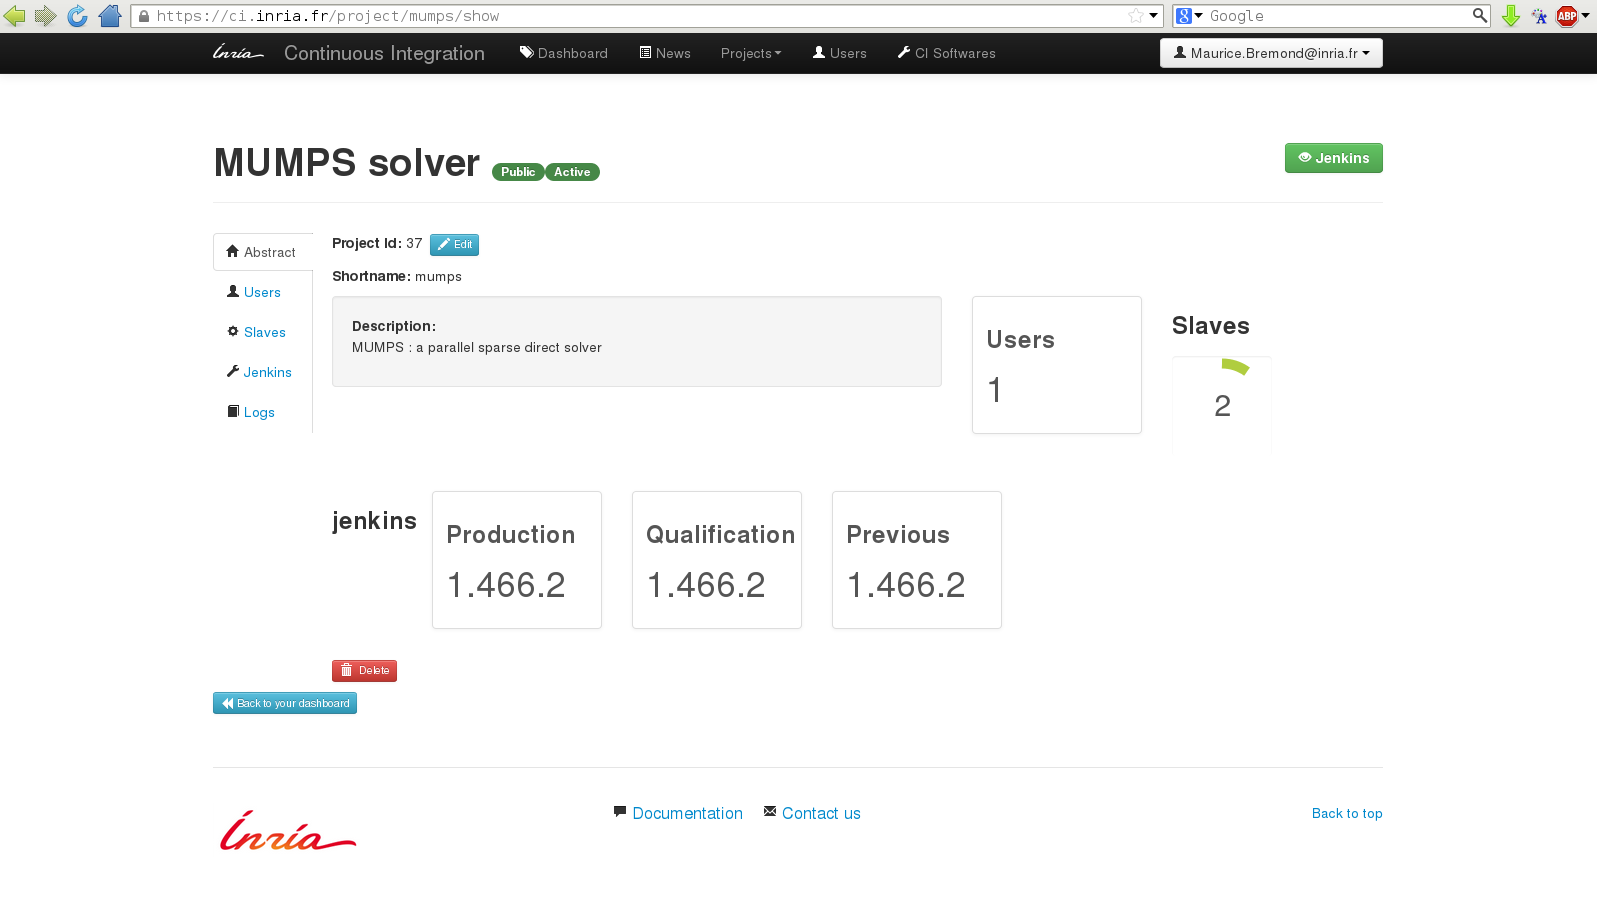
\includegraphics[width=1.2\textwidth] {images/ci-project.png}};
  \end{tikzpicture}
\end{frame}

\begin{frame}{Interface haut niveau pour les machines virtuelles associées}

\begin{tikzpicture}
 \node[] (project)  {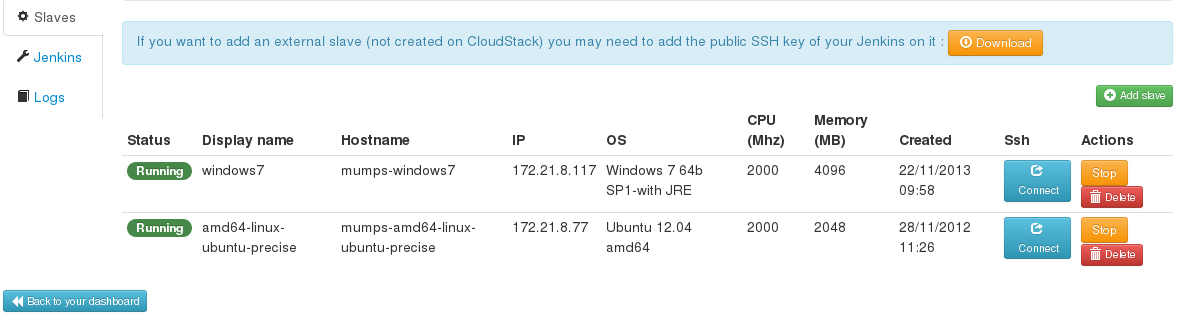
\includegraphics[width=.9\textwidth] {images/ci-slaves.png}};
\end{tikzpicture}
\end{frame}

\begin{frame}{Création d'une nouvelle machine}
  \begin{tikzpicture}
    \node[] (project)  {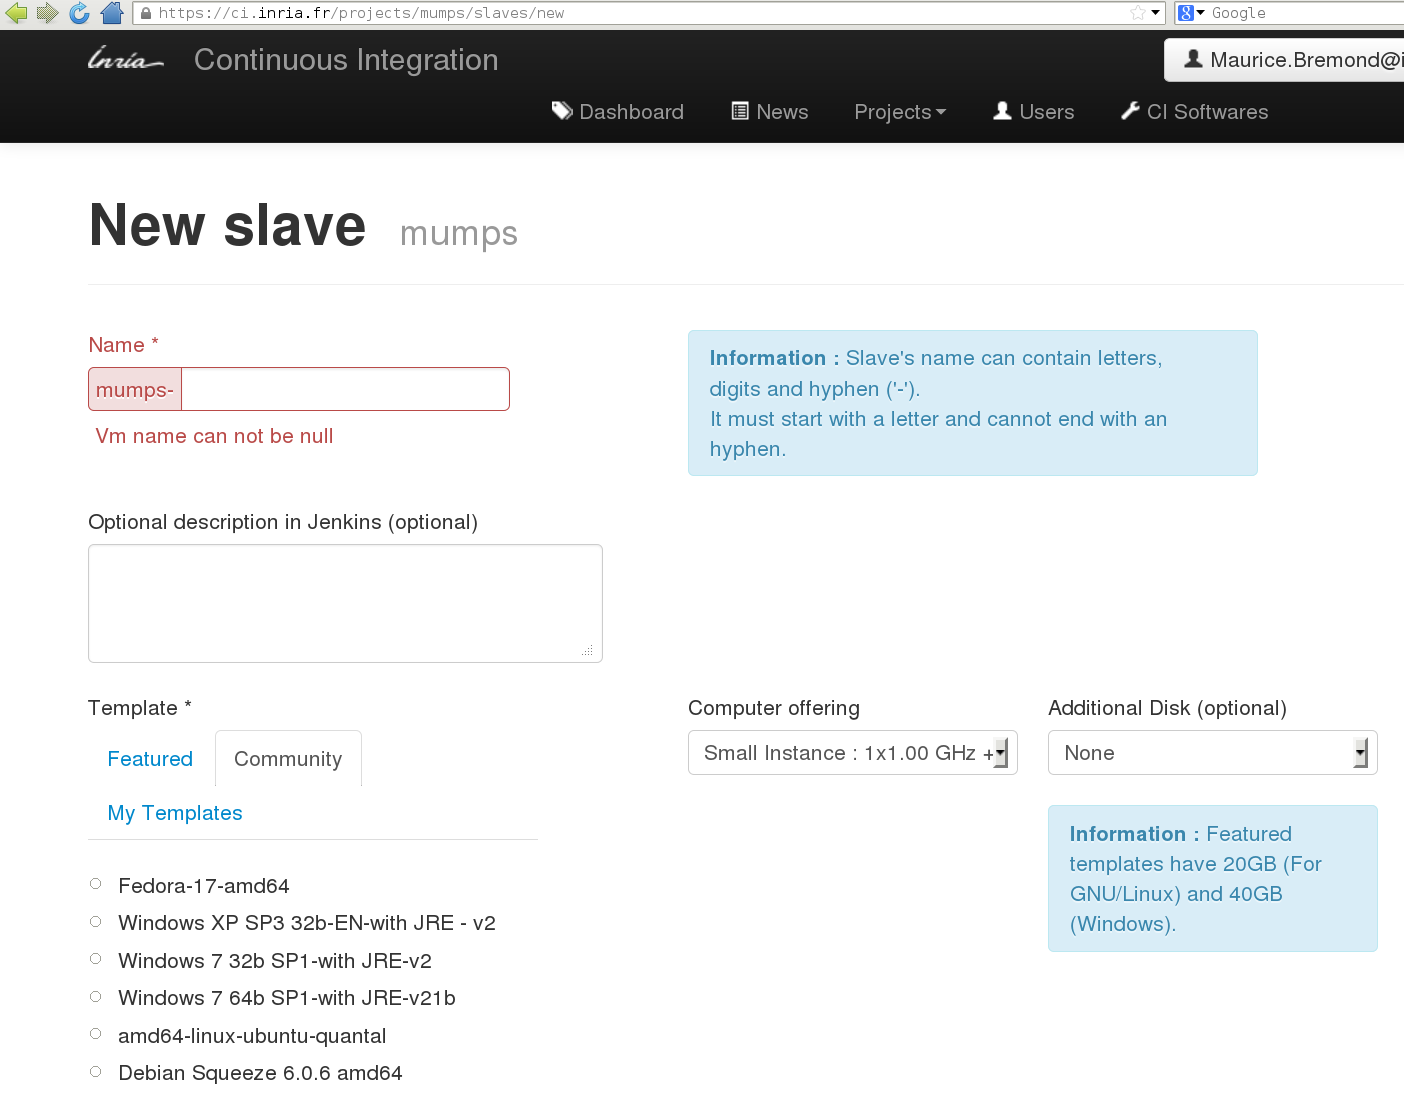
\includegraphics[width=.9\textwidth] {images/new-slave.png}};
  \end{tikzpicture}
\end{frame}


\begin{frame}{Accès direct au gestionnaire sous-jacent : cloudstack}
  \begin{tikzpicture}
    \node[] (project)  {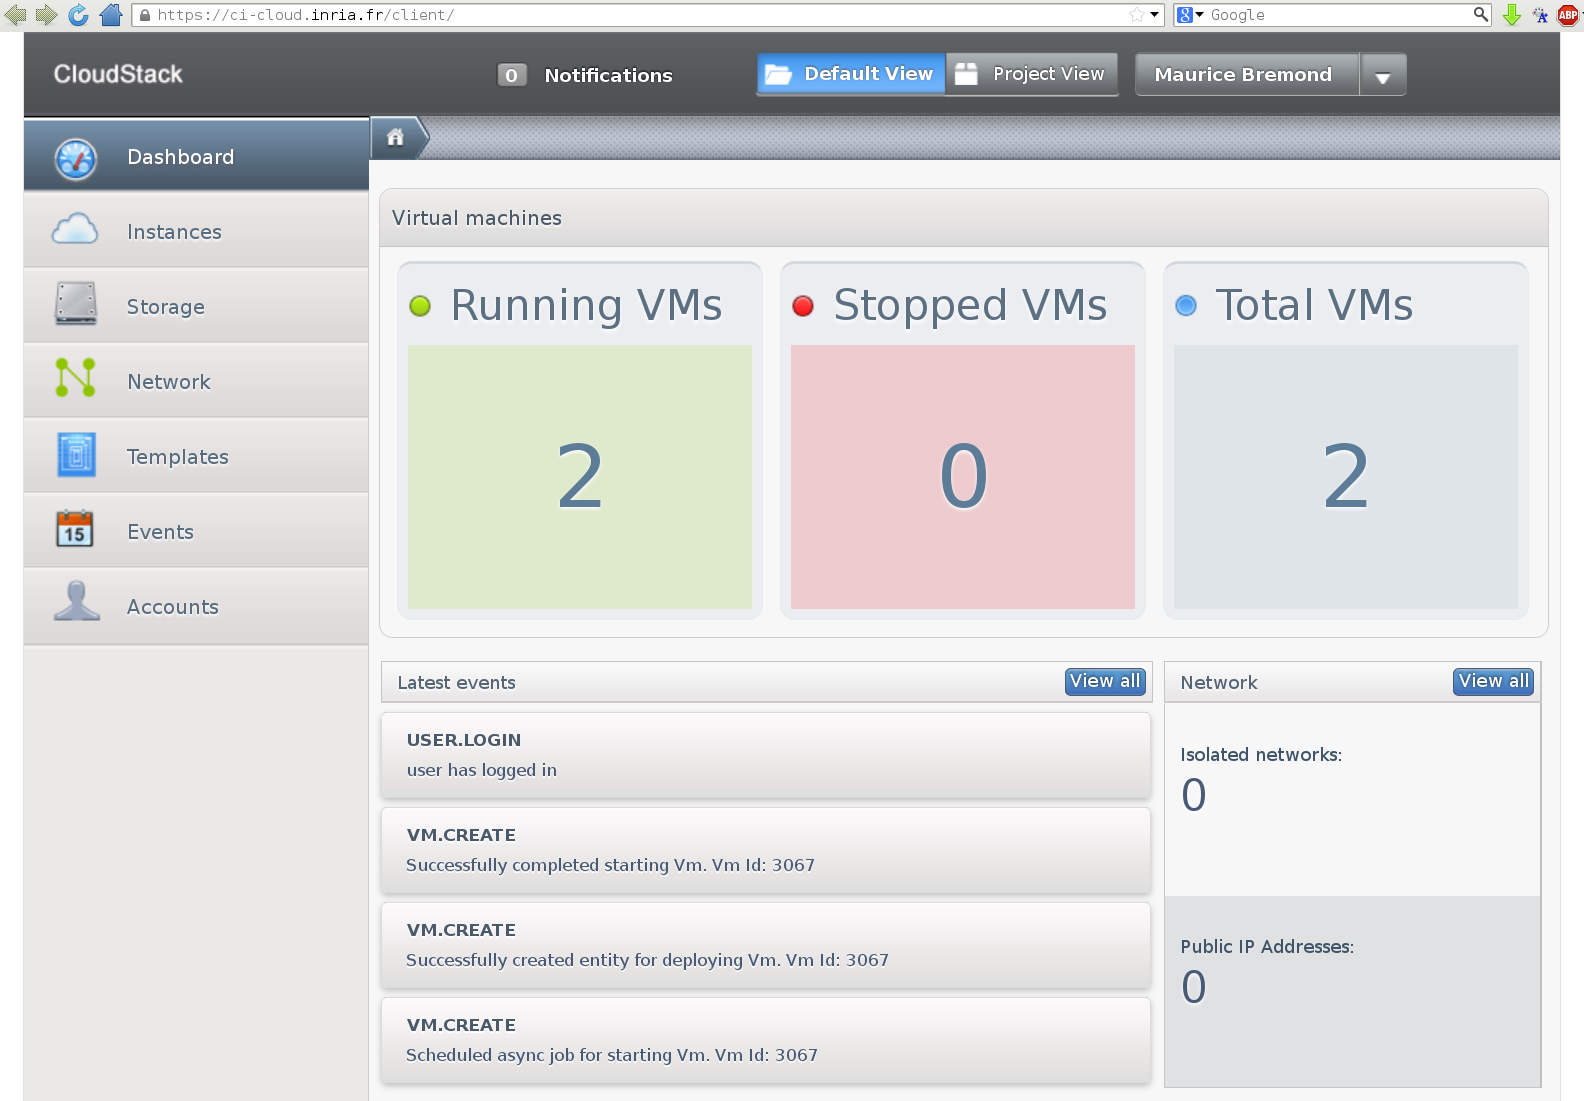
\includegraphics[width=1.2\textwidth] {images/cloudstack-main.png}};
  \end{tikzpicture}
\end{frame}

\begin{frame}{Accès direct au gestionnaire sous-jacent : cloudstack/machine}
\begin{tikzpicture}
 \node[] (windows_conf)  {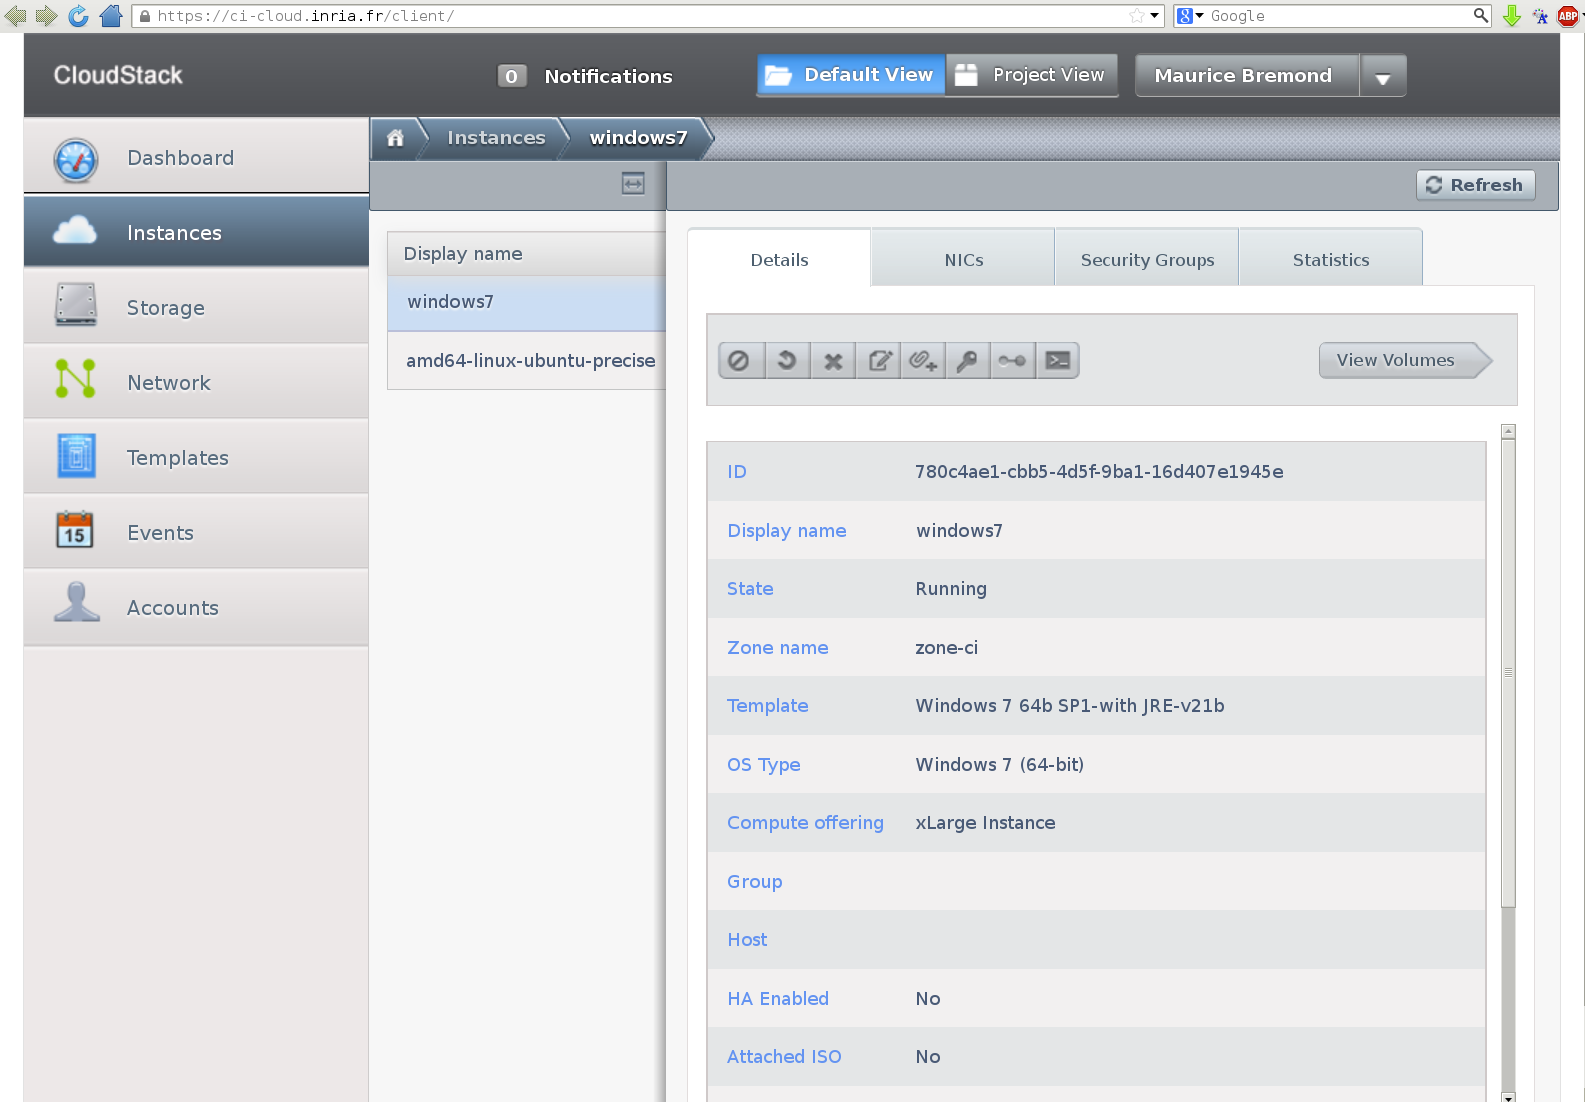
\includegraphics[width=1.2\textwidth] {images/cloudstack-windows-conf.png}};
 \node[draw,ellipse,minimum height=.8cm,minimum width=.8cm,thick,color=red] at (2.3,1.6) (select) {};
 \node[draw,rectangle,thick,color=red,rounded corners=2pt] at (-4,-0.4) (windows_desktop) {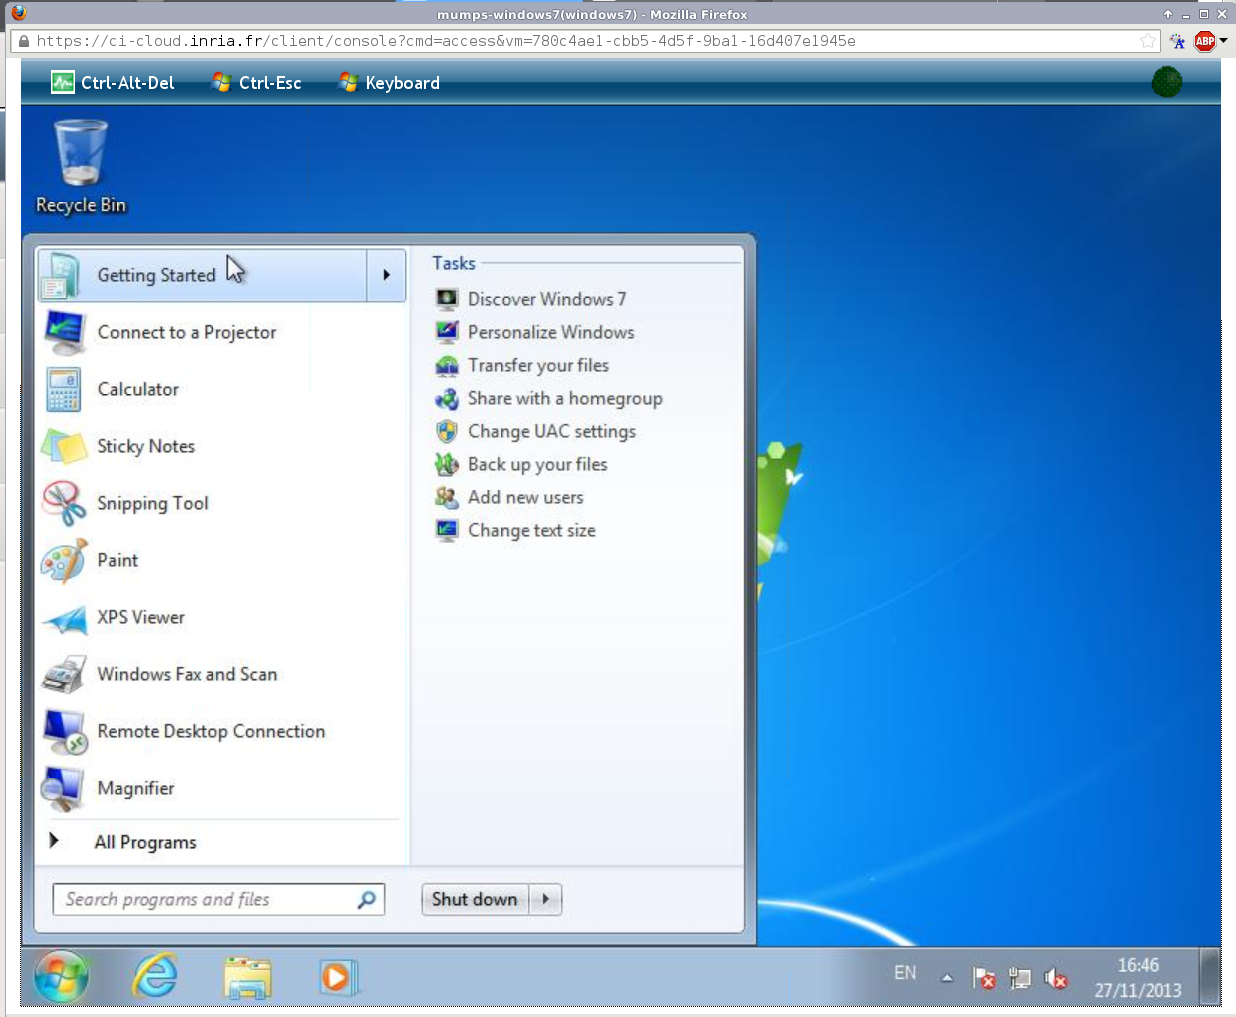
\includegraphics[width=.4\textwidth] {images/cloudstack-windows-desktop.png}};
 \path[->, thick, color=red] (select.south) edge [bend left] (windows_desktop.east);
\end{tikzpicture}
\end{frame}


% Retour d'expérience
% *******************
\inriaswitchcolors{green}
\section{Un retour d'expérience}
\frame{\tableofcontents[currentsection]
  \note{Vous avez besoin d'intégration continue\\}
  \note{Exemple mon expérience personnelle}
}

\subsection{Contexte de développement}
\tocsubsection{\note{Justifié de le faire pour moi, vous reconnaître sur certains points}}

\subsubsection{FIT Equipex - Future Internet of Things}
\begin{frame}{\subsubsecname} %{\subsecname}
  \note[item]{Equipex: 'equipement excellence' projet FR}
  \note[item]{Future Internet of Thing.}
  \note[item]{}
  \note[item]{L'internet des objets, c'est quoi?}
  \note[item]{Un pot de fleur, avec capteur humidité, message sur téléphone}
  \note[item]{}
  \note[item]{plusieurs plateformes}
  \note[item]{Durée de 10 ans}
  \note[item]{}
  \note[item]{IOT-LAB - description slide suivant}

  \begin{center}
    \begin{tabular}{ l l }
      
\includegraphics[width=0.2\textwidth]{images/logo_invest_avenir} &
      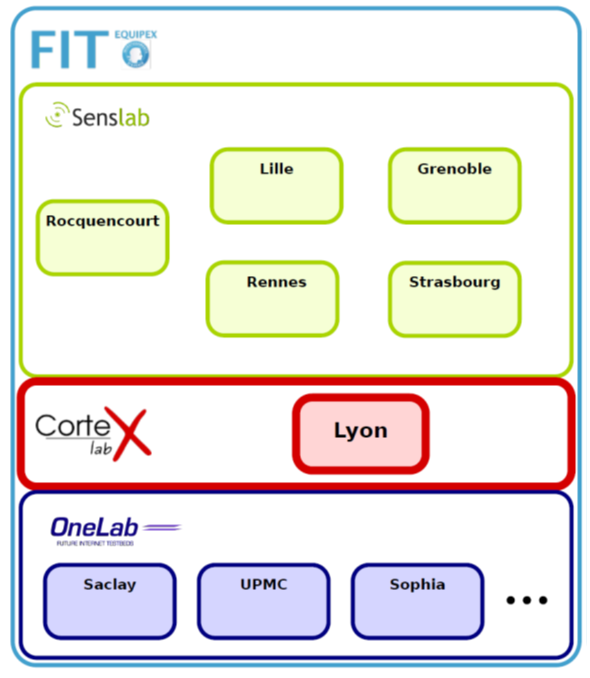
\includegraphics[width=0.5\textwidth]{images/fit_equipex} \\
    \end{tabular}
  \end{center}
\end{frame}


\subsubsection{Plateforme de réseau de capteurs: FIT IoT-LAB}
\begin{frame}{\subsubsecname} %{\subsecname}
  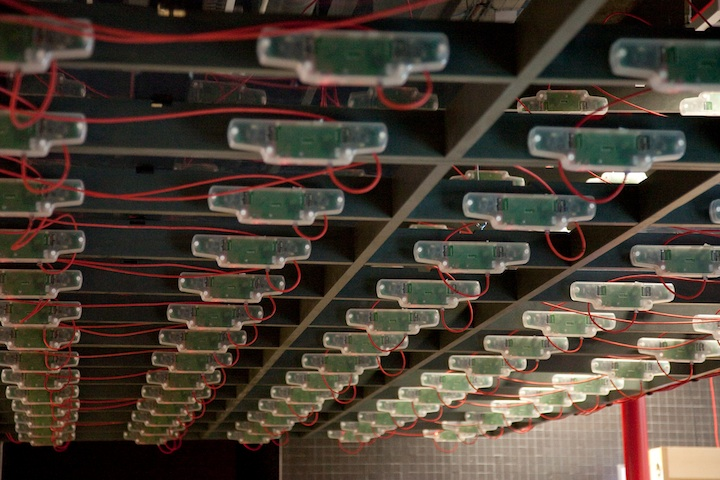
\includegraphics[width=\textwidth]{images/senslab_nodes}
  \note[item]{IoT-LAB: réseaux de capteurs 'objets connectés' à large échelle, 3000}
  \note[item]{Objets qui communiquent courte distance, et joignable depuis l'internet}
  \note[item]{Faible consommation, bande passante faible}
  \note[item]{}
  \note[item]{1 minute pour en programmer 3 sur son PC, 30 secondes pour en programmer 1000 avec IoT-LAB}
  \note[item]{}
  \note[item]{Mis à disposition des chercheurs}
  \note[item]{2 générations de capteurs}
\end{frame}

\begin{frame}{\subsubsecname} %{\subsecname}
  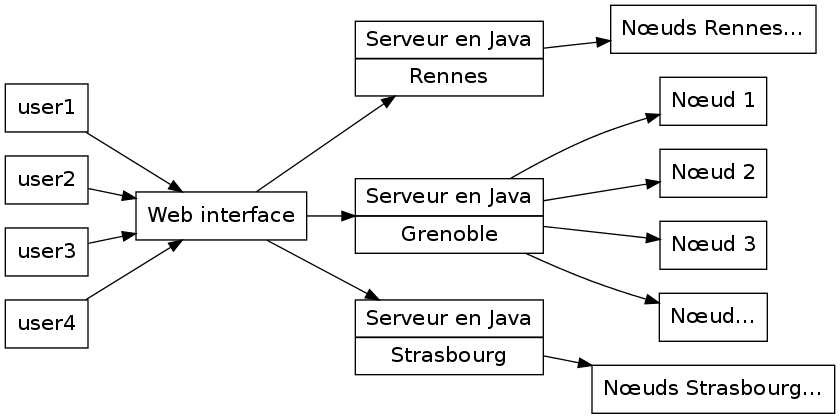
\includegraphics[width=\textwidth]{images/fit_architecture}
  \note{Exemple d'un chercheur voulant expérimenter sur les réseaux de capteurs}
  \note[item]{Se connecter sur l'interface web}
  \note[item]{Réserver un grand nombre de nœuds capteurs (3k dispos)}
  \note[item]{Déployer des programmes dessus}
  \note[item]{Interragir avec eux par connection série}
  \note[item]{Monitorer leur fonctionnement, conso, radio}
\end{frame}


\subsubsection{Un nœud capteur IoT-LAB}
\begin{frame}{\subsubsecname} %{\subsecname}
  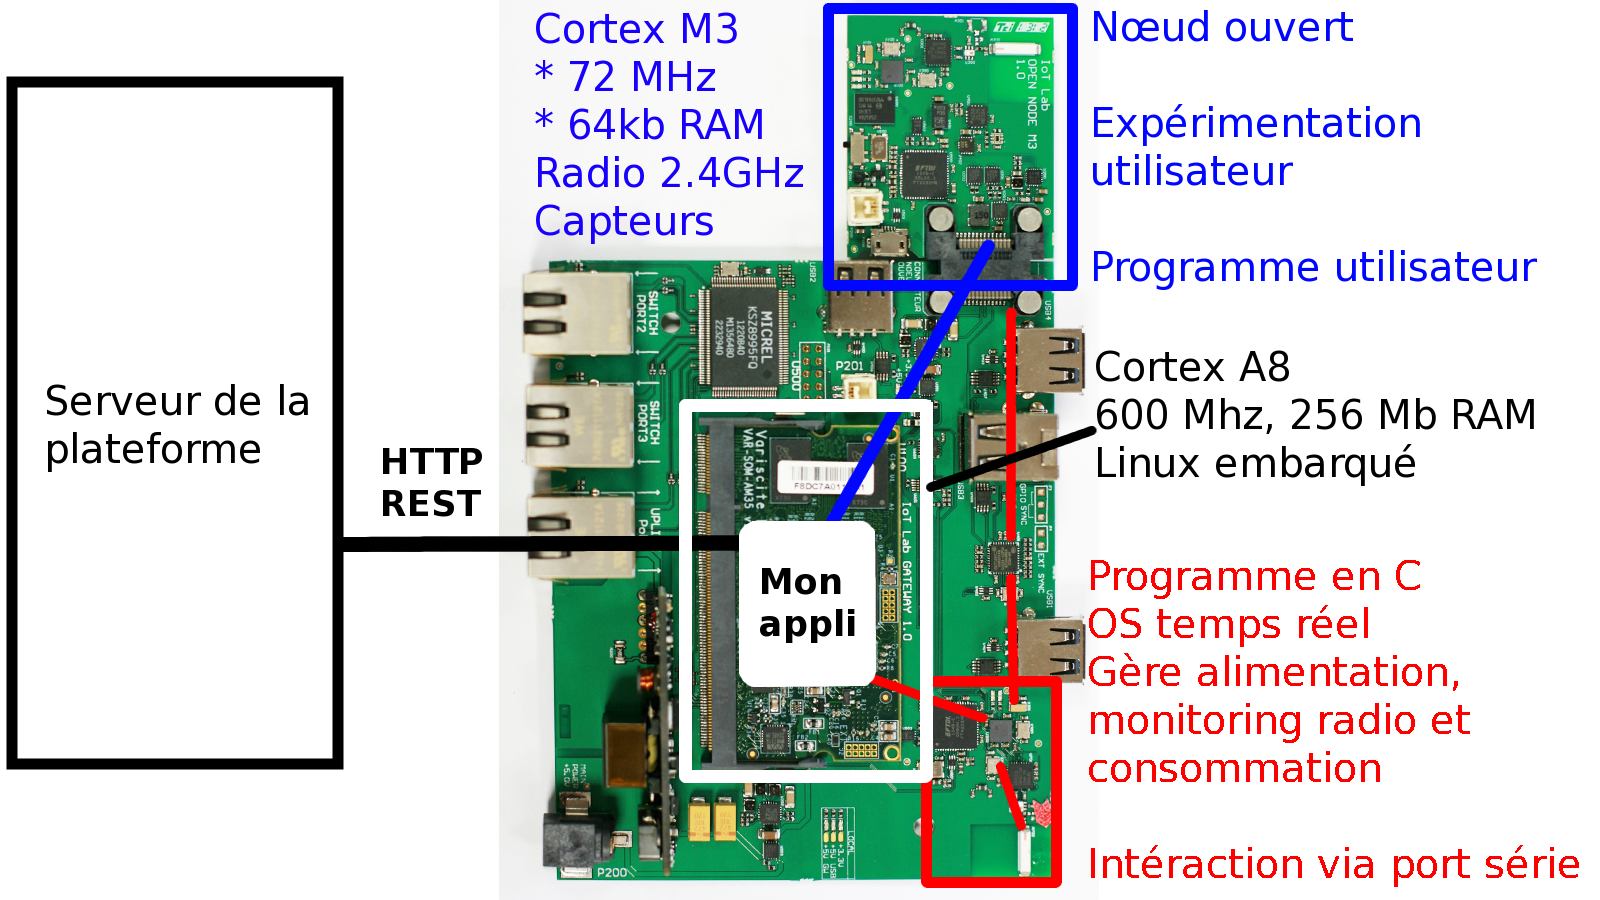
\includegraphics[width=\textwidth]{images/gateway_m3_annote}
\end{frame}

\subsubsection{Contexte de l'application}
\begin{frame}{\subsubsecname} %{\subsecname}
  \begin{itemize}
    \item Python + C (+ outils compilés externes)
    \item Application mise en production (QoS)
    \item Exécution sur une carte ARM avec Linux embarqué (perf...)
    \item Intéractions extérieures
    \item multithread, multiprocess
  \end{itemize}
\end{frame}


\subsubsection{Pourquoi avoir mis place de l'intégration continue}
\begin{frame}{\subsubsecname} %{\subsecname}
  \begin{itemize}
    \item Sources d'erreurs non déterministes
      \note[item]{Dépendance à du matériel}
      \note[item]{Dépendance à des programmes qui ne sont pas sur la même machine}
      \note[item]{Multithread et multiprocess}
      \note[item]{}
    \item Logiciel final doit être fiable
      \note[item]{service 24/7}
      \note[item]{Coût d'un bug: Debug, mise à jour}
      \note[item]{Large échelle, proba d'apparition d'un bug}
      \note[item]{}
    \item J'avais envie d'essayer
    \item La chose qui m'a décidée…
  \end{itemize}
\end{frame}

\subsubsection{J'avais besoin d'un seul test}
\begin{frame}[fragile]{\subsubsecname} %{\subsecname}
  \setbeamercovered{transparent}

  \begin{verbatim}

  def thread_redirection(self):
      while not self.stop:
          self.proc = subprocess.Popen(['socat', ...)
          self.proc.wait()
          if 0 != self.proc.returncode:
              # Gestion de l'erreur

    def stop(self):
        while self.is_alive():
        self.proc.terminate()
        time.sleep(0.1)

  \end{verbatim}

  \onslide <2-> Test sur carte: '\texttt{ImportError: No module named arpgarse}'

  \note{Code testé sur mon PC, sur le serveur, sur la carte finale, marche sur les 3}
\end{frame}



%
%  Outils mis en place
%
\subsection{Outils mis en place}
\tocsubsection{
  \note[item]{Juste une overview, un exemple}
  \note[item]{Quelques possibilité et contraintes}
  \note[item]{En utilisant ci.inria.fr}
}

\subsubsection{Mise en place d'un \texttt{build}}
\begin{frame}{\subsubsecname} % {\subsecname}
  \setbeamercovered{transparent}

  \onslide <1-> Script \textbf{automatisé} et \textbf{autotesté} qui va réaliser la validation du logicel.
  \\ ~\\
  \begin{itemize}
    \item <2-> Compilation
    \item <2-> Exécution des tests (unitaires et fonctionnels)
    \item <2-> Inspection automatique de code
      \begin{itemize}
        \item <2-> évaluation de la qualité de code par analyse statique
      \end{itemize}
    \item <2-> Génération de documentation
      \begin{itemize}
        \item <2-> Rapports de tests (couverture de code)
        \item <2-> Documentation technique
      \end{itemize}
  \end{itemize}
\end{frame}


\subsubsection{Exemple d'un test Python}
\begin{frame}[fragile]{\subsubsecname} % {\subsecname}

\begin{verbatim}
import unittest

class WidgetTestCase(unittest.TestCase):
    def setUp(self):
        self.widget = Widget('The widget')

    def tearDown(self):
        self.widget.dispose()
        self.widget = None

    def test_default_size(self):
        self.assertEqual(self.widget.size(), (50,50),
                         'incorrect default size')

    def test_resize(self):
        self.widget.resize(100,150)
        self.assertEqual(self.widget.size(), (100,150),
                         'wrong size after resize')

\end{verbatim}
\end{frame}

\subsubsection{Présentation des outils}
\begin{frame}{Outils mis en place}

  Gestionnaire de versions: \texttt{git} \\ ~ \\

  \begin{tabular}{ l | l l | p{3.5cm} }
    Language         & \texttt{Python}     & \texttt{C}    & Utiisation dans Jenkins \\ \hline
    Script de build  & \texttt{setuptools} & \texttt{Make} & Bash~shell, \texttt{EnvInject} \texttt{virtualenv}\\
    Compilation      & ~                   & \texttt{gcc}  & ~ \\
    Tests            & \texttt{nose}, \texttt{unittest}, \texttt{mock}
                     & \texttt{gtest} \texttt{(C++)}
                     & Junit, Chuck Norris\\
    Couverture       & \texttt{nose-xcover}
                     & \texttt{gcov}, \texttt{gcovr}
                     & Cobertura \\
   Qualité de code  & \texttt{pylint}, \texttt{pep8} & ~  & Violations \\
                   ~ & ~  & ~ & \\
    Lignes de code   &  $3000$        &  $1500$  &  $0$  \\
    Lignes de tests  &  $1600 + 400$  &  $1300$  &  $0$  \\
% 1600 tests U + 400 tests intégration
    Lignes de build  &  $300$         &  $170$   &  $50$ \\

    \note[item]{Gestion de version, partagée avec d'autres projets}
    \note[item]{Correspondance entre outils mis en place et Jenkins, \textbf{fichiers générés}}
    \note[item]{Types d'outils les uns après les autres}
    \note[item]{Pylint remplace compilation python}
    \note[item]{}
    \note[item]{1600 tests U + 400 tests intégration}
    \note[item]{SQLite 3.8 == 1084 * plus de tests que de code 84k source (hors blank et commentaires)}
  \end{tabular}
\end{frame}


\subsubsection{Jenkins}
\begin{frame}{Présentation outils}{Jenkins}
  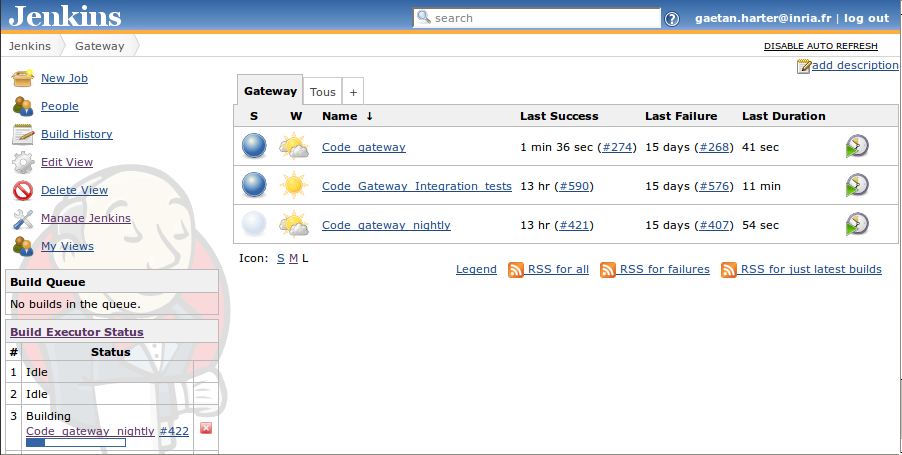
\includegraphics[width=\linewidth]{images/jenkins}
  \note[item]{2 types}
  \note[item]{Sur carte cible \textbf{Thales}}
  \note[item]{Lancement des tests, à la main et toute les nuits}
\end{frame}

\begin{frame}{Configuration d'un build}{Jenkins}
  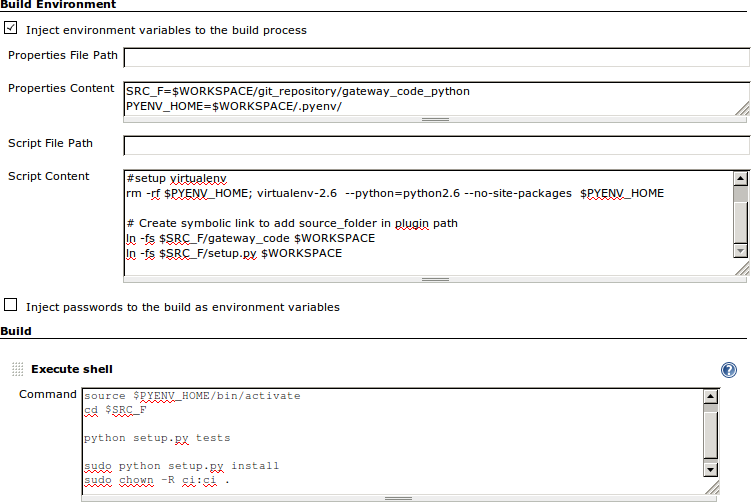
\includegraphics[width=\linewidth]{images/build_configuration}
\end{frame}


\begin{frame}{Cobertura}{Jenkins}
        % Pour moi, l'outil le plus important (après Chuck Norris forcément)
  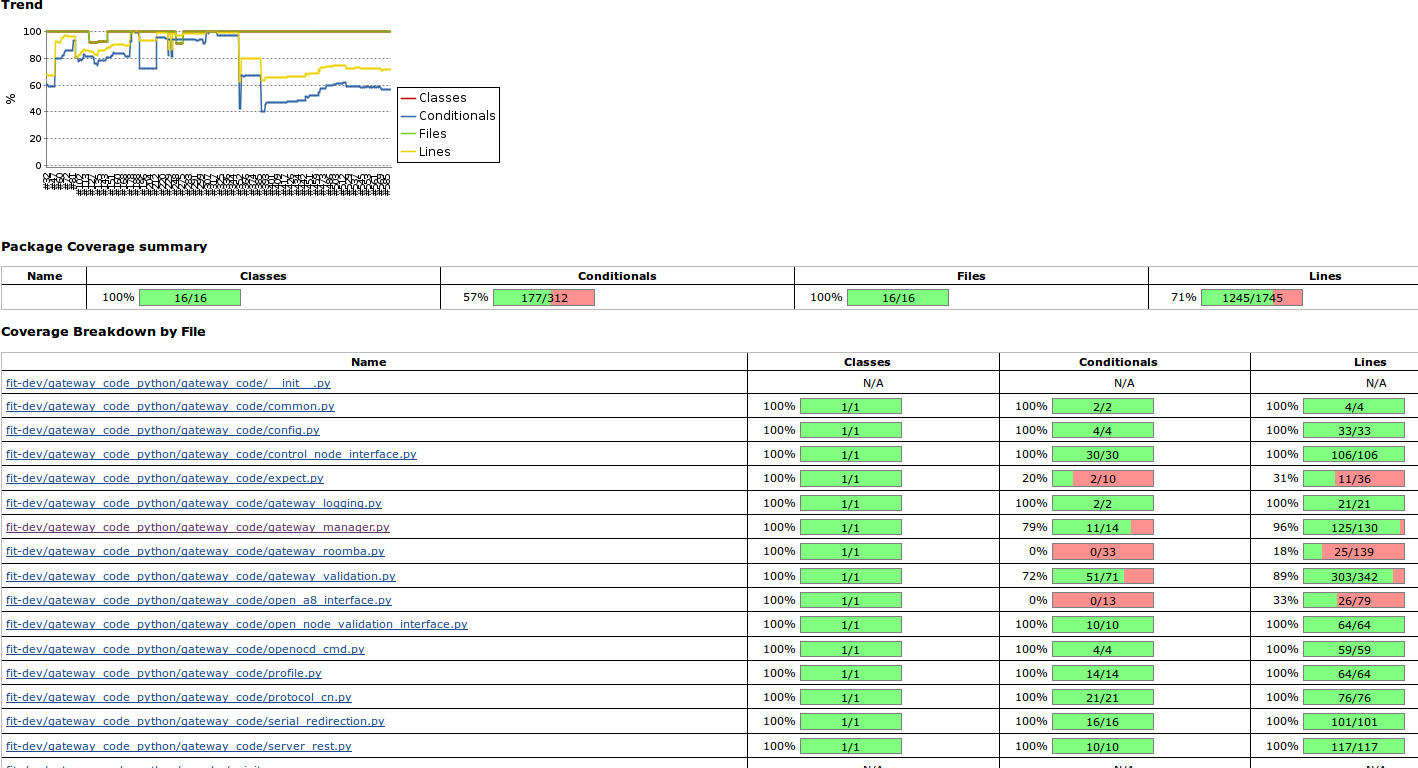
\includegraphics[width=\linewidth]{images/cobertura}\\
\end{frame}
\begin{frame}{Junit - Violations}{Jenkins}
  \begin{center}
        % Juste pour montrer
    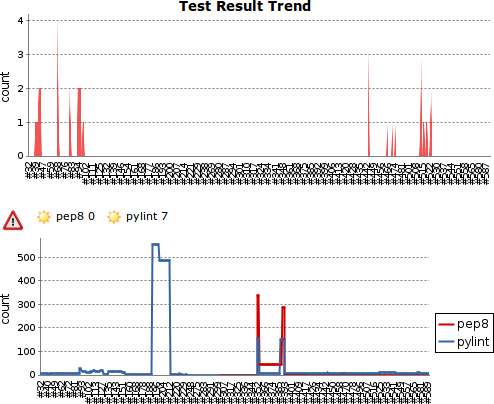
\includegraphics[height=0.8\textheight]{images/junit_violations}\\
  \end{center}
\end{frame}
\begin{frame}{Chuck Norris}{Jenkins}
  % Le plus important des plugins
  \begin{center}
    \begin{tabular}{ l |l }
      Build KO & Build OK \\ \hline
        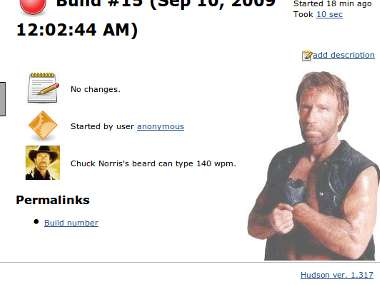
\includegraphics[height=4cm]{images/chuck_full} &
      
\includegraphics[height=4cm]{images/chuck_happy}
        %
\includegraphics[height=4cm]{images/chuck_angry}
      \\
    \end{tabular}
  \end{center}
  Chuck Norris Facts:
  \begin{itemize}
    \item Chuck Norris can unit test an entire application with a single assert.
    \item Chuck Norris can divide by zero.
    \item ...
  \end{itemize}
\end{frame}




\subsection{Bilan}
\tocsubsection


\subsubsection{Développement logiciel}
\begin{frame}{\subsubsecname}{\subsecname}
  \note{GROS SLIDE}

  \begin{itemize}
    \item Mise en place d'un script de \texttt{build}
      \note[item]{Procédure de test, même 1 seul test}
      \note[item]{Procédure simple dans un script}
      \note[item]{}
    \item Tests nombreux et lancés en continu
      \note[item]{Gestion des cas d'erreurs}
      \note[item]{Détection de problèmes tot (perf réimplèm en C}
      \note[item]{simplification de l'implem}
      \note[item]{dev itératif}
      \note[item]{Detection d'erreurs rares}
      \note[item]{}
    \item Couverture de code
      \note[item]{Même si $<100\%$, savoir ce qui est 'validé' et ce qui ne l'est pas}
      \note[item]{}
    \item Qualité de code
      \note[item]{Python: Remplace la phase de compilation (vérification syntaxique)}
      \note[item]{Détection statique d'erreurs}
      \note[item]{Standardisation de la mise en forme, lisibilité (PEP8)}
      \note[item]{}
  \end{itemize}
  Maîtrise et confiance dans le logiciel développé
\end{frame}

\subsubsection{Bilan personnel}
\begin{frame}{\subsubsecname}{\subsecname}
  \setbeamercovered{transparent}
  \onslide <1-> Postulat: Un bon développeur veux faire du bon code.
  \begin{itemize}
    \item <2-> Retours positifs après premières utilisations
    \item <2-> Confort dans le développement
    \item <2-> Découverte de beaucoup d'outils
    \item <2-> Maîtrise des languages et leur écosystème
    \item <2-> Apprends à mieux coder (Chuck and Guido approved)
  \end{itemize}

  \note[item]{Un bon développeur veux savoir faire du bon code}
  \note[item]{Code fonctionnel}
  \note[item]{Découverte}
  \note[item]{Amélioration}
  \note[item]{Je code mieux maintenant}

  \note[item]{Guido van Rossum}
  \note[item]{}
  \note[item]{Je peux tester}
\end{frame}

\subsubsection{Voies d'amélioration}
\begin{frame}{\subsubsecname}{\subsecname}
  \begin{itemize}
    \item Passer les configurations Jenkins dans des scripts versionnés
    \item Grouper Python et C dans le build python
    \item Inclusion d'autres développeurs
    \item 100\% de couverture de code
  \end{itemize}
\end{frame}


\begin{frame}{The End}
  Merci d'avoir écouté.
\end{frame}


\end{document}
